\documentclass[a4paper]{article}

\usepackage[brazilian]{babel} %Para traduzir os textos
\usepackage[utf8]{inputenc} %Para poder usar acentos
\usepackage[a4paper]{geometry} %Para ajustar a parte geometrica da folha
\geometry{verbose,tmargin=2cm,bmargin=3cm,lmargin=1.2cm,rmargin=2cm} %Parte de margens
\setlength{\parindent}{0.5cm}
\usepackage{wrapfig} %Biblioteca Matematica/Grafica
\usepackage{mathptmx} %Biblioteca Matematica/Grafica
\renewcommand{\ttdefault}{mathptmx} %Biblioteca Matematica/Grafica
\usepackage{amsmath} %Biblioteca Matematica/Grafica
\usepackage{amssymb} %Biblioteca Matematica/Grafica
\usepackage[11pt]{moresize}% different letters sizes
\usepackage{float}% enables accurate location of tables
\usepackage{caption}% to make personalized captions
\usepackage{graphicx} %Para inclusão de imagens
\usepackage{amsfonts}
\usepackage[T1]{fontenc}

\makeatletter
\providecommand{\tabularnewline}{\\} %define

\title{Máquina de Atwood \\ Experimento 4} % main title
\author{F 229 \\ \textsc{Grupo 1}}
\date{XX de XX, 2014}


\begin{document} % actually starts the document here
\maketitle

% members of the group
\begin{center}
	\begin{tabular}{l r l}
		Integrantes:\\\\
		 Henrique Noronha Facioli & RA: 157986 \\
		 Guilherme Lucas da Silva & RA: 155618 \\
		 Beatriz Sechin Zazulla & RA: 154779 \\
		 Lucas Alves Racoci & RA: 156331 \\
		 Isadora Sophia Garcia Rodopoulos & RA :158018 \\
	\end{tabular}
\end{center}

\newpage{}

\section{Resumo}
Neste experimento, estudamos uma \emph{Máquina de Atwood}, um sistema físico que consiste de: um cilindro de latão funcionando como polia, ou seja, com liberdade de girar em torno de um eixo fixo; um fio que será considerado leve - ou seja, com massa irrelevante -, inestensível - isto é, inelástico; dois corpos (1 e 2) que são pendurados na polia por meio do fio anteriormente citado, onde:
\begin{itemize} 
	\item O corpo 1 consiste de um sub-corpo de massa ${m}_{1}$ e mais $n_{1}$ de $5$ sub-corpos; 
	\item O corpo 2 consiste de um sub-corpo de massa ${m}_{2}$ e mais $n_{2}$ de $5$ sub-corpos; 
	\item Os valores de $n_{1}$ e $n_{2}$ são tais que $n_{1}+n_{2}=5$; 
	\item As massas dos corpos 1 e 2 serão chamadas respectivamente de $m_{1}$ e $m_{2}$.
\end {itemize} 

Sabemos que a diferença entre as massas dos dois corpos gera um torque não nulo na polia, o que nos permite estudar seu Momento de Inércia $I_{0}$ e a aceleração da grávidade $g$, através da fórmula a seguir:

\begin{align}
\Delta_m=\cfrac{2h}{gR^{2}}(I+MR^{2})\ensuremath{\cfrac{1}{t^{2}}}+\cfrac{\tau_{a}}{gR}
\end{align}


\section{Objetivo}
Este experimento tem como principal objetivo o estudo da máquina de Atwood através da determinação do momento de inércia da polia e do torque da força de atrito, possibilitados a partir da manipulação de um sistema inserido no modelo de estudo.


\section{Procedimentos e coleta de dados}

Na realização deste experimento foram utilizados os seguintes materiais: 
\begin{enumerate} 
	\item Polia de latão com eixo;
	\item Barbante;
	\item Conjunto de discos metálicos;
	\item Trena;
	\item Paquímetro;
	\item Balança de precisão;
	\item Cronômetro.
 \end {enumerate} 

\begin{figure}[!ht]
	\centering
	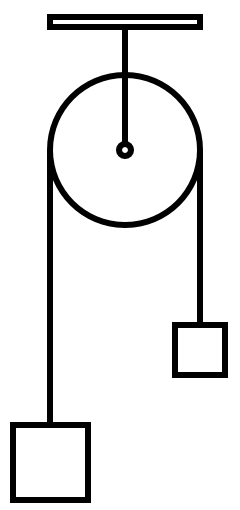
\includegraphics[scale=0.25]{Atwood_machine.jpg}
	\caption{Montagem do experimento}
\end{figure}

Para a montarmos a Máquina de Atwood, prendemos dois pesos de suspensão, $m_1$ e $m_2$ com um fio (barbante de algodão), e o encaixamos sobre um cilindro de latão de modo que o lado de maior peso fizesse o lado de menor peso descer.Para essas duas massas $m_1$ e $m_2$, variávamos um conjunto de 5 pequenas massas ($a , b ,  c ,  d ,  e$) de modo que $m_1$ sempre estivesse com o maior peso maior que $m_2$ mas que o conjunto sempre mantivesse a massa $M$ total constante.
Depois disso, medimos a distância $h$ do solo até a massa elevada (que em nosso caso será $m_1$),e para cada variação de massa $\Delta_{m} = {m_1} - {m_2}$ mediamos 5 vezes o tempo de queda com um cronômetro.

\begin{table}[!ht]
	\begin{centering}
	\caption{Massas experimentalmente medidas}
	\par\end{centering}
	\centering{}%
	\begin{tabular}{|c|c|}
	\hline 
	Nome & Massa $[Kg]$\tabularnewline		\hline 
	$a$ & $(9,6\pm0,1)\centerdot10^{-3}$\tabularnewline		\hline 
	$b$ & $(1,97\pm0,01)\centerdot10^{-2}$\tabularnewline	\hline 
	$c$ & $(1,93\pm0,01)\centerdot10^{-2}$\tabularnewline	\hline 
	$d$ & $(9,3\pm0,1)\centerdot10^{-3}$\tabularnewline \hline 
	$e$ & $(9,8\pm0,1)\centerdot10^{-3}$\tabularnewline	\hline 
	$\widetilde{m}_{1}$ & $(8,934\pm0,001)\centerdot10^{-1}$\tabularnewline 	\hline 
	$\widetilde{m}_{2}$ & $(8,934\pm0,001)\centerdot10^{-1}$\tabularnewline 	\hline 
	\end{tabular}
\end{table}

\begin{table}[!ht]
	\begin{centering}
	\caption{Massas obtidas experimentalmente}
	\par\end{centering}
	\centering{}%
	\begin{tabular}{|c|c|c|c|c|c|}
	\hline 
	N & 1 & 2 & 3 & 4 & 5\tabularnewline	\hline 
	$m_{1}$$[Kg]$ & $\widetilde{m_{1}}+a+b+c+d+e$ & $\widetilde{m_{1}}+a+b+c+d$ & $\widetilde{m_{1}}+a+b+c$ & $\widetilde{m_{1}}+a+b+c+e$ & $\widetilde{m_{1}}+a+c+e$\tabularnewline		\hline 
	$m_{1}$$[Kg]$ & $(9,611\pm0,002)\cdot10^{-1}$ & $(9,513\pm0,002)\cdot10^{-1}$ & $(9,420\pm0,002)\cdot10^{-1}$ & $(9,518\pm0,002)\cdot10^{-1}$ & $(9,321\pm0,002)\cdot10^{-1}$\tabularnewline	\hline 
	$m_{2}$$[Kg]$  & $\widetilde{m_{2}}$ & $\widetilde{m_{2}}+e$ & $\widetilde{m_{2}}+d+e$$(\pm)\cdot10^{-1}$ & $\widetilde{m_{2}}+d$ & $\widetilde{m_{2}}+b+d$\tabularnewline	\hline 
	$m_{2}$$[Kg]$ & $(8,934\pm0,001)\cdot10^{-1}$ & $(9,032\pm0,001)\cdot10^{-1}$ & $(9,125\pm0,001)\cdot10^{-1}$ & $(9,027\pm0,001)\cdot10^{-1}$ & $(9,224\pm0,002)\cdot10^{-1}$\tabularnewline	\hline 
	$\Delta m$ & $(6,77\pm0,03)\cdot10^{-2}$ & $(4,81\pm0,03)\cdot10^{-2}$ & $(2,95\pm0,03)\cdot10^{-2}$ & $(4,91\pm0,03)\cdot10^{-2}$ & $(9,7\pm0,3)\cdot10^{-3}$\tabularnewline	\hline 
	\end{tabular}
\end{table}

\begin{table}[!ht]
	\begin{centering}
	\caption{Tempos de queda medidos experimentalmente para cada $\Delta m$}
	\par\end{centering}
	\centering{}%
	\begin{tabular}{|c|c|c|c|c|c|}
	\cline{2-6} 
	\multicolumn{1}{c|}{} & $\Delta m_{1}$ & $\Delta m_{2}$ & $\Delta m_{3}$ & $\Delta m_{4}$ & $\Delta m_{5}$\tabularnewline	\hline 
	$t_{1}\pm\sigma_{t_{inst}}$$[s]$ & $2,66\pm0,01$ & $3,22\pm0,01$ & $4,28\pm0,01$ & $3,25\pm0,01$ & $7,72\pm0,01$\tabularnewline		\hline		$t_{2}\pm\sigma_{t_{inst}}$$[s]$ & $2,56\pm0,01$ & $3,25\pm0,01$ & $4,28\pm0,01$ & $3,22\pm0,01$ & $7,32\pm0,01$\tabularnewline		\hline 
	$t_{3}\pm\sigma_{t_{inst}}$$[s]$ & $2,68\pm0,01$ & $3,12\pm0,01$ & $4,19\pm0,01$ & $3,19\pm0,01$ & $7,78\pm0,01$\tabularnewline		\hline 
	$t_{4}\pm\sigma_{t_{inst}}$$[s]$ & $2,59\pm0,01$ & $3,25\pm0,01$ & $4,18\pm0,01$ & $3,19\pm0,01$ & $7,56\pm0,01$\tabularnewline		\hline 
	$t_{5}\pm\sigma_{t_{inst}}$$[s]$ & $2,65\pm0,01$ & $2,28\pm0,01$ & $4,22\pm0,01$ & $3,22\pm0,01$ & $7,53\pm0,01$\tabularnewline		\hline 
	\end{tabular}
\end{table}
	

\section{Análise dos resultados}

Para determinar o momento de inercia $I$ e o torque da força de atrito $\tau_{a}$ através da equação (1), precisamos escolher quem será $X$ e $Y$ e depois, se necessário linearizar a fórmula, mas nesse caso, se fizermos: $\underset{Y}{\underbrace{\Delta m}}=\underset{a}{\underbrace{\cfrac{2h}{gR^{2}}(I+MR^{2})}}\underset{X}{\underbrace{\ensuremath{\cfrac{1}{t^{2}}}}}+\underset{b}{\underbrace{\cfrac{\tau_{a}}{gR}}}$ a equção já fica em sua forma linearizada. Assim, variando $\Delta m$ e $t$ obtemos os valores de $I$ e $\tau_{a}$ a partir de $a$, $b$, $h$, $g$, $R$, e $M=m_{1}+m_{2}$.
Mas para obter $a$ e $b$ precisa-se realizar o Método dos Mínimos Quadrados, e para isso precisamos achar um valor de $t$ para cada valor de $\Delta m$ calculada na Tabela 2.


Para o calculo do erro em $m_{i}$:

\begin{align}
	\sigma_{m_{i}}^{2}={\displaystyle \sum_{k=1}^{n_{i}}\left(\left(\cfrac{\partial m_{i}}{\partial m_{k}}\right)^{2}\centerdot(\sigma_{m_{k}})^{2}\right)}
\end{align}

mas todos os $\sigma_{m_{k}}$'s são iguais, pois se trata do erro experimental, então:

$$\sigma_{m_{i}}^{2}={\displaystyle \sum_{k=1}^{n_{i}}\left(\left(\cfrac{\partial m_{i}}{\partial m_{k}}\right)^{2}\centerdot(\sigma_{m})^{2}\right)}={\displaystyle \sum_{k=1}^{n_{i}}\left(\left(\cfrac{\partial m_{i}}{\partial m_{k}}\right)^{2}\right)}\centerdot(\sigma_{m})^{2}$$

Sabemos também que $m_{i}={\displaystyle \sum_{j=1}^{t}(m_{j})}$ portanto:

$$\cfrac{\partial m_{i}}{\partial m_{k}}=\cfrac{\partial}{\partial m_{k}}\left({\displaystyle \sum_{j=1}^{t}(m_{j})}\right)={\displaystyle \sum_{j=1}^{t}\left(\cfrac{\partial m_{j}}{\partial m_{k}}\right)=1}$$

porque $ \cfrac{\partial m_{j}}{\partial m_{k}}=0 $, exceto quando $j=k$,quando $\cfrac{\partial m_{j}}{\partial m_{k}}=\cfrac{\partial m_{k}}{\partial m_{k}}=1$

Assim:

$$\sigma_{m_{i}}^{2}={\displaystyle \sum_{k=1}^{n_{i}}\left(\left(\cfrac{\partial m_{i}}{\partial m_{k}}\right)^{2}\right)}\centerdot(\sigma_{m})^{2}=\sigma_{m_{i}}^{2}={\displaystyle \sum_{k=1}^{n_{i}}\left(1^{2}\right)}\centerdot(\sigma_{m})^{2}={\displaystyle n}\centerdot(\sigma_{m})^{2}\Leftrightarrow$$

\begin{align}
\sigma_{m_{i}}=\sigma_{m}\sqrt{n_{i}}
\end{align}

Para $\Delta m$ o resultado é ainda mais interessante: $\Delta m=m_{1}-m_{2}$ portanto o erro é 

$$\sigma_{\Delta m}^{2}=\sigma_{m_{1}}^{2}\left(\cfrac{\partial\Delta m}{\partial m_{1}}\right)^{2}+\sigma_{m_{2}}^{2}\left(\cfrac{\partial\Delta m}{\partial m_{2}}\right)^{2}=\sigma_{m_{1}}^{2}\left(1\right)^{2}+\sigma_{m_{2}}^{2}\left(-1\right)^{2}=\sigma_{m_{1}}^{2}+\sigma_{m_{2}}^{2}=\sigma_{m}^{2}\centerdot n_{1}+\sigma_{m}^{2}\centerdot n_{2}=\sigma_{m}^{2}(n_{1}+n_{2})$$

\begin{align}
\sigma_{\Delta m}=\sigma_{m}\sqrt{n_{1}+n_{2}}=\sigma_{m}\sqrt{n}
\end{align}

que é um valor constante porque o número de massas utilizadas não muda.

Agora temos que achar um valor único de $t$ para associar com cada valor de $\Delta m$. Como fizemos 5 medidas de $t$ pra cada $\Delta m$, então para achar o valor único pra $t$ e seu erro devemos fazer:

$$t=\overline{t}\pm\sigma_{t}$$ 

onde $\overline{t}$ é a média aritmética $\cfrac[r]{\overset{{\scriptstyle 5}}{\underset{{\scriptstyle i=1}}{\sum}}t_{i}}{5}$; e $\sigma_{t}$ é o erro total $\sqrt{{\displaystyle \sigma_{t_{inst}}^{2}+\sigma_{t_{estat}}^{2}}}=\sqrt{{\displaystyle \sigma_{t_{inst}}^{2}+}\cfrac[r]{1}{5}\cfrac[l]{1}{4}\overset{{\scriptstyle 5}}{\underset{{\scriptstyle i=1}}{\sum}}(t_{i}+\overline{t})^{2}}$. Utilizando os valores da Tabela 3 , obtemos os seguintes valores para $t=\overline{t}\pm\sigma_{t}$

\begin{table}[!ht]
	\begin{centering}
	\caption{Valores da média do tempo para cada valor de $\Delta M$}
	\par\end{centering}
	\centering{}%
	\begin{tabular}{|c|c|c|c|c|c|}
	\cline{2-6} 
	\multicolumn{1}{c|}{} & $\Delta m_{1}$ & $\Delta m_{2}$ & $\Delta m_{3}$ & $\Delta m_{4}$ & $\Delta m_{5}$\tabularnewline	\hline
	$t=\overline{t}\pm\sigma_{t}$$[s]$ & $2,63\pm0,02$ & $3,22\pm0,03$ & $4,21\pm0,02$ & $3,21\pm0,02$ & $7,58\pm0,08$\tabularnewline	\hline
	\end{tabular}
\end{table}

Agora temos uma relação bem clara entre $\Delta m$ e $t$:

Fazendo $X=\cfrac{1}{t^{2}}$ o erro fica

$$\sigma_{X}^{2}=\sigma_{t}^{2}\left(\cfrac{\partial X}{\partial t}\right)^{2}\Leftrightarrow\sigma_{X}=\left|-2t^{-3}\sigma_{t}\right|=\cfrac{2}{t^{3}}\sigma_{t}$$
No entanto, não será usado porque o Métodos dos Mínimos Quadrados que está sendo usado não considera erro em $X$.
Fazendo $Y=\Delta m$ o erro será:

\begin{align}
\sigma_{Y}^{2}=\sigma_{\Delta m}^{2}\Leftrightarrow\sigma_{Y}=\sigma_{\Delta m}
\end{align}

Fazendo o Método dos Mínimos Quadrados com esses dados obtem-se o gráfico da reta:

\begin{wrapfigure}{o}{0.5\columnwidth}%
	\caption{Gráfico de $\Delta m\times\frac{1}{t^{2}}$ COMPLETAR}
	
\end{wrapfigure}%

Cujos coeficientes angular e linear são respectivamente:

\begin{eqnarray*}
\begin{cases}
a=\cfrac{2h}{gR^{2}}(I+MR^{2}) & (angular)\\
b=\cfrac{\tau_{a}}{gR} & (linear)
\end{cases} & \Leftrightarrow & \begin{cases}
agR^{2} & =2h(I+MR^{2})\\
bgR & =\tau_{a}
\end{cases}\Leftrightarrow
\end{eqnarray*}


\begin{eqnarray*}
\Leftrightarrow & \begin{cases}
\cfrac[r]{agR^{2}}{2h}=I+MR^{2}\\
\tau_{a}=bgR
\end{cases}\Leftrightarrow & \begin{cases}
I=\cfrac[r]{agR^{2}}{2h}-MR^{2}\\
\tau_{a}=bgR
\end{cases}
\end{eqnarray*}


Para calcular os erros tem-se:

$$ \sigma_{I}^{2}=\sigma_{a}^{2}\left(\cfrac[r]{\partial I}{\partial a}\right)^{2}+\sigma_{g}^{2}\left(\cfrac[r]{\partial I}{\partial g}\right)^{2}+\sigma_{R}^{2}\left(\cfrac{\partial I}{\partial R}\right)^{2}+\sigma_{h}^{2}\left(\cfrac[r]{\partial I}{\partial h}\right)^{2}+\sigma_{M}^{2}\left(\cfrac{\partial I}{\partial M}\right)^{2} $$

\begin{align}
\sigma_{I}=\sqrt{\sigma_{a}^{2}\left(\cfrac[r]{gR^{2}}{2h}\right)^{2}+\sigma_{g}^{2}\left(\cfrac[r]{aR^{2}}{2h}\right)^{2}+\sigma_{R}^{2}\left(\cfrac{Rag}{h}-2RM\right)^{2}+\sigma_{h}^{2}\left(\cfrac[r]{-agR^{2}}{2h^{2}}\right)^{2}+\sigma_{M}^{2}\left(-R^{2}\right)^{2}}\end{align}

Já para o torque da força de atrito o processo é um pouco mais simples:


$$\sigma_{\tau_{a}}^{2}=\sigma_{b}^{2}\left(\cfrac[r]{\partial I}{\partial b}\right)^{2}+\sigma_{g}^{2}\left(\cfrac[r]{\partial I}{\partial g}\right)^{2}+\sigma_{h}^{2}\left(\cfrac[r]{\partial I}{\partial h}\right)^{2}$$

\begin{align}
\sigma_{\tau_{a}}=\sqrt{(\sigma_{b}gh)^{2}+(b\sigma_{g}h)^{2}+(bg\sigma_{h})^{2}}
\end{align}

Portanto:

$$I=\overline{I}\pm\sigma_{I}=(2,00\pm0,07)\centerdot10^{-1}Kg\centerdot m^{2}$$

$$\tau_{a}=\overline{\tau_{a}}\pm\sigma_{\tau_{a}}=(1,5\pm0,2)\centerdot10^{-2}N\centerdot m$$

\section{Conclusão}

Para termos um parâmetro de comparação podemos usar a massa e o raio do cilindro de metal para calcular o valor do Momento de Inércia teórico
$I_{T}$e comparar com o que obtivemos experimentalmente:

$$I_{T}=M_{polia}\centerdot R^{2}=2,05330\centerdot(4,995\centerdot10^{-1})^{2}=2,5615\centerdot10^{-1}$$

Para o erro, como não foi informado o erro para $M_{polia}$, supomos somente o erro instrumental de $10^{-4}$$Kg$ da mesma balança analítica:

$$
\sigma_{I_{T}}^{2}=\sigma_{M_{polia}}^{2}\left(\cfrac{\partial I}{\partial M_{polia}}\right)^{2}+\sigma_{R}^{2}\left(\cfrac{\partial I}{\partial R}\right)^{2}
$$

\begin{align}
\sigma_{I_{T}}=\sqrt{\sigma_{M_{polia}}^{2}\left(R^{2}\right)^{2}+\sigma_{R}^{2}\left(2MR\right)^{2}}
\end{align}

Ou seja, temos que:

$$I_{T}=(2,6\pm0,5)\centerdot10^{-1}Kg\centerdot m^{2}$$

$$I=(2,00\pm0,07)\centerdot10^{-1}Kg\centerdot m^{2}$$

Se usarmos todas as casas decimais e não somente as mostradas aqui temos:

$$
I_{T}-\sigma_{I_{T}}=2,05\centerdot10^{-1}Kg\centerdot m^{2}\leq2,07\centerdot10^{-1}Kg\centerdot m^{2}=I+\sigma_{I}
$$

Nosso resultado pode ser considerado dentro do esperado por esse tipo de parâmetro, mas não pelo parâmetro formalizado em aula, que não considera as casas decimais de erro não significativos. Alguns fatores podem justificar o valor longe, ainda que muito perto do esperado, tais como:
\begin{itemize}
	\item O imprecisão do tempo de disparo do cronômetro
	\item O fio não ser inextensível;
	\item O escorregamento do fio no cilindro de latão;
\end{itemize}

O que pode ser feito para resolver esses problemas numa próxima realização é:
\begin{itemize}
	\item Considerar o fio extensível.
	\item Usar uma superfície que tenha um alto coeficiente de atrito estático com o fio;
\end{itemize}

\end{document}